In the previous chapters, we considered how propagating quanta of radiation scatter on different quantum systems. In this chapter, we are instead going to consider how we can mediate entanglement between two 
spatially separated matter qubits. This is an interesting topic as it plays a vital role in numerous quantum technology applications, such as quantum repeaters (and ultimately quantum networks) \cite{}. Photons can here mediate interaction between qubits, and entanglement can be achieved through bell state measurements on beamsplitters.

When the two emitters are identical and operate without dephasing noise, the emitted photons are indistinguishable, and their wavefunctions exhibit a complete overlap. Due to the Hong Ou Mandel effect\cite{MANDEL}, the "which path information" is thus erased when combined on a beamsplitter, and consequently, entanglement can be achieved. However, in realistic scenarios, differences between the emitters introduce variations in the respective wavefunctions of the emitted photons, leading to imperfect overlaps. The photons become distinguishable, and the fidelity of the entanglement is reduced. 

To address this challenge, various protocols have been proposed that try to maximize the fidelity of the entanglement while still keeping a high success probability. There are numerous ways to simulate these protocols, and typically a master equation approach can be applied \cite{Barrett2004EfficientOptics}.

In this chapter, we will show how we can simulate such protocols using the time-binned photon formalism. The approach enables straightforward calculation of the success probabilities, the photon indistinguishability, and the protocol fidelity since we have access to the complete wavefunction of the emitted photons. 

\section{Entanglement of two emitters}

In ref. \cite{Barrett2004EfficientOptics} they propose a scheme to entangle two distant matter qubits. The qubits consist of three states: Two longlived lover excited states $\ket{\uparrow}$ and $\ket{\downarrow}$ and one excited state $\ket{e}$ that can undergo the transition $\ket{e} \rightarrow \ket{\downarrow}$ by emitting a photon. The transition $\ket{e} \rightarrow \ket{\uparrow}$ is not permitted due to selection rules. Each qubit is placed inside a cavity where the cavity mode matches the frequency of the transition $\ket{e} \rightarrow \ket{\downarrow}$.

Before we go over the scheme proposed in ref. \cite{Barrett2004EfficientOptics}, we consider the evolution of an excited state in both qubits. We thus have the initial state $\ket{\psi(t=0)} = \ket{e,0,\emptyset}_a \ket{e,0,\emptyset}_b$, where $\ket{e,0,\emptyset}_{a/b}$ denotes an excited qubit $\ket{e}$, an empty cavity $\ket{0}$, and an empty waveguide $\ket{\emptyset}$ at site a/b . Assuming sufficient time $t_{wait}$ has passed, all excitations will have leaked out of the emitter/cavity system and into the waveguide. We can thus describe the system at this point as:
\begin{equation}
     \ket{\psi(t_{wait})} = \sum_k \sum_j \xi_a(t_k)\xi_b(t_j) 
 w_{k,a}^\dagger w_{j,b}^\dagger \ket{\downarrow,0,\emptyset}_a \ket{\downarrow,0,\emptyset}_b
\end{equation}
where $\xi_a(t_k)$ and $\xi_b(t_j)$ are the amplitudes of the emission from site $a$ and $b$ at time $t_k$ and $t_j$, respectively and $w_{k,a/b}^\dagger$ the creation operator of a photon in waveguide $a/b$ in time-bin $k$.  

If the emitted photons subsequently interfere on a beamsplitter, the waveguide operators transform as $w_{k,a}^\dagger \rightarrow \frac{1}{\sqrt{2}} \left [ w_{k,a}^\dagger + w_{k,b}^\dagger \right ]$ and $w_{k,b}^\dagger \rightarrow \frac{1}{\sqrt{2}} \left [ w_{k,a}^\dagger - w_{k,b}^\dagger \right ]$. The state after the interaction is then: 
\begin{align}
    \ket{\psi(t_{wait})}  &\xrightarrow{BS} \frac{1}{2} \sum_k \sum_j \xi_a(t_k)\xi_b(t_j) \left [w_{k,a}^\dagger+w_{k,b}^\dagger \right ] \left [w_{j,a}^\dagger-w_{j,b}^\dagger \right ]  \ket{\downarrow,0,\emptyset}_a \ket{\downarrow,0,\emptyset}_b \\
    &=  \frac{1}{2} \sum_k \sum_j \xi_a(t_k)\xi_b(t_j) \left [w_{k,a}^\dagger w_{j,a}^\dagger - w_{k,a}^\dagger w_{j,b}^\dagger + w_{k,b}^\dagger w_{j,a}^\dagger - w_{k,b}^\dagger w_{j,b}^\dagger \right ] \ket{\downarrow,0,\emptyset}_a \ket{\downarrow,0,\emptyset}_b
\end{align}

The probability of detecting two photons in waveguide $a$ at time $t_i$ and $t_j$ after the beamsplitter interaction can then be calculated by using the projector:
\begin{equation}
P_{aa}(t_i,t_j) = w_{i,a}^\dagger w_{j,a}^\dagger \ket{\downarrow,0,\emptyset}_a \ket{\downarrow,0,\emptyset}_b \bra{\downarrow,0,\emptyset}_a \bra{\downarrow,0,\emptyset}_b w_{i,a} w_{j,a}    
\end{equation}
where the probability is then given as (we here leave out $\ket{\downarrow,0}$ since they just fall out and immediately notice that all terms are zero except the one containing $w_{k,a}^\dagger w_{j,a}^\dagger$):
\begin{align}
    &\bra{\psi(t_{wait})} P_{aa}(t_i,t_j) \ket{\psi(t_{wait})} = \\
    &\frac{1}{4} \sum_{k,l,m,n} \xi_a^*(t_k)\xi_b^*(t_l) \xi_a(t_m)\xi_b(t_n) \bra{\emptyset}_a \bra{\emptyset}_b w_{j,a} w_{k,a} w_{i,a}^\dagger w_{j,a}^\dagger  \ket{\emptyset}_a \ket{\emptyset}_b \bra{\emptyset}_a \bra{\emptyset}_b w_{i,a} w_{j,a} w_{l,a}^\dagger w_{m,a}^\dagger  \ket{\emptyset}_a \ket{\emptyset}_b \\
    & = \frac{1}{4} \sum_{k,l,m,n}  \xi_a^*(t_k)\xi_b^*(t_l) \xi_a(t_m)\xi_b(t_n) (\delta_{il}\delta_{jk}+\delta_{ik}\delta_{jl})(\delta_{im}\delta_{in}+\delta_{in}\delta_{im}) \\
    &= \frac{1}{4} (\xi_a^*(t_i)\xi_b^*(t_j) + \xi_a^*(t_j)\xi_b^*(t_i))(\xi_a(t_i)\xi_b(t_j) +\xi_a(t_j)\xi_b(t_i)) = \abs{\xi_a(t_i)\xi_b(t_j) +\xi_a(t_j)\xi_b(t_i)}^2
\end{align}
The total probability of observing two photons in waveguide $a$ $P_aa$ is then the sum of all the above projections two-time projections:
\begin{equation}
   P_{aa} = \frac{1}{4} \sum_i \sum_j \abs{( \xi_a(t_i)\xi_b(t_j) + \xi_a(t_j)\xi_b(t_i))}^2
\end{equation}

Similarly, we would have the probability of observing one photon in waveguide $a$ and one photon in waveguide $b$ $P_{ab}$:
\begin{equation}
   P_{ab} = \frac{1}{4} \sum_i \sum_j \abs{( \xi_a(t_i)\xi_b(t_j) - \xi_a(t_j)\xi_b(t_i))}^2
\end{equation}
If the two emitted photons are identical, $\xi_a(t_i)\xi_b(t_j) =  \xi_a(t_j)\xi_b(t_i)$ and we would thus never observe two photons in different waveguides after the beamsplitter. This is the Hong-Ou-Mandel effect. 

The total probability of having detector + clicking thus is:

\begin{equation}
    P(D_+) =  \sum_j \sum_m \frac{1}{2} \abs{\frac{1}{2} ( \xi_a(t_j)\xi_b(t_m) + \xi_a(t_m)\xi_b(t_j))}^2 + \abs{ \frac{1}{2} ( -\xi_a(t_m) \xi_b(t_j) +\xi_a(t_j) \xi_b(t_m))}^2
\end{equation}


Detecting a second photon again leads to:

\begin{align}
    D_\pm \ket{\psi(t_{wait})} &\rightarrow D_\pm D_\pm \ket{\psi(t_{wait})} \\
    & = \frac{1}{2} \sum_k \sum_j \left( \pm \xi_a(t_k)\xi_b(t_j)  \ket{\downarrow, 0, \emptyset}_a \ket{\downarrow,0,\emptyset}_b \pm \xi_a(t_j)\xi_b(t_k) \ket{\downarrow,0,\emptyset}_a \ket{\downarrow,0,\emptyset}_b \right )   
\end{align}

From this it is evident that if $\xi_a(t)=\xi_b(t)$ for all times then observing a click in two different detectors is not possible (as expected). 

The intital state is, however, slithgly more complicated since the initial state is the following entangled state:

\begin{equation}
    \ket{\psi} = \frac{1}{2}(\ket{e}_a+\ket{\uparrow}_a)\ket{0,\emptyset}_a(\ket{e}_b+\ket{\uparrow}_b)\ket{0,\emptyset}_b
\end{equation}

After sufficient time, the excited states $\ket{e}_{a/b}$ has decayed and emitted a photon into the waveguide. We here have the (un-normalized) state:

\begin{align}
    \ket{\psi} &= \sum_k  \xi_b(t_k) \ket{\uparrow,0,\emptyset}_a \ket{\downarrow,0,1_k}_b + \sum_k \xi_a(t_k) \ket{\downarrow,0,1_k}_a \ket{\uparrow,0,\emptyset}_b \\
    & + \sum_k \sum_j \xi_a(t_k)\xi_b(t_j) \ket{\downarrow,0,1_k}_a\ket{\downarrow,0,1_j}_b + \ket{\uparrow,0,\emptyset}_a\ket{\uparrow,0,\emptyset}_b
\end{align}

After the first detection, we thus have:

\begin{align}
    \ket{\psi} \rightarrow D_\pm \ket{\psi} &=  \sum_k \xi_a(t_k) \ket{\downarrow,0,\emptyset}_a \ket{\uparrow,0,\emptyset}_b \pm \xi_b(t_k) \ket{\uparrow,0,\emptyset}_a \ket{\downarrow,0,\emptyset}_b \\
    &+ \sum_k \sum_j \xi_a(t_k)\xi_b(t_j) \ket{\uparrow,0,\emptyset}_a\ket{\uparrow,0,1_j}_b \pm \ket{\uparrow,0,1_k}_a\ket{\uparrow,0,\emptyset}_b 
\end{align}

In the paper, they then take into account the fact that realistic photo detectors cannot capture two photons arriving in a quick succession. They simulate this by allowing no more information to be gained, claiming that the resulting state would be:

\begin{equation}
    \rho \propto \ket{\psi_\pm} \bra{\psi_\pm} + \ket{\uparrow,0,\emptyset}_a\ket{\uparrow,0,\emptyset}_b \bra{\uparrow,0,\emptyset}_a\bra{\uparrow,0,\emptyset}_b
\end{equation}

where $\ket{\psi_\pm} = \ket{\downarrow,0,\emptyset}_a \ket{\uparrow,0,\emptyset}_b \pm \ket{\uparrow,0,\emptyset}_a \ket{\downarrow,0,\emptyset}_b$. Ideally, we would like not to simulate density matrices, and perhaps this is where the montecarlo trajectory comes into the picture. Do we split up in two paths from here. One where we have projected onto the entangled state and one where we project onto everything else?



\section{Entanglement heralding}
\begin{figure}[H]
    \centering
    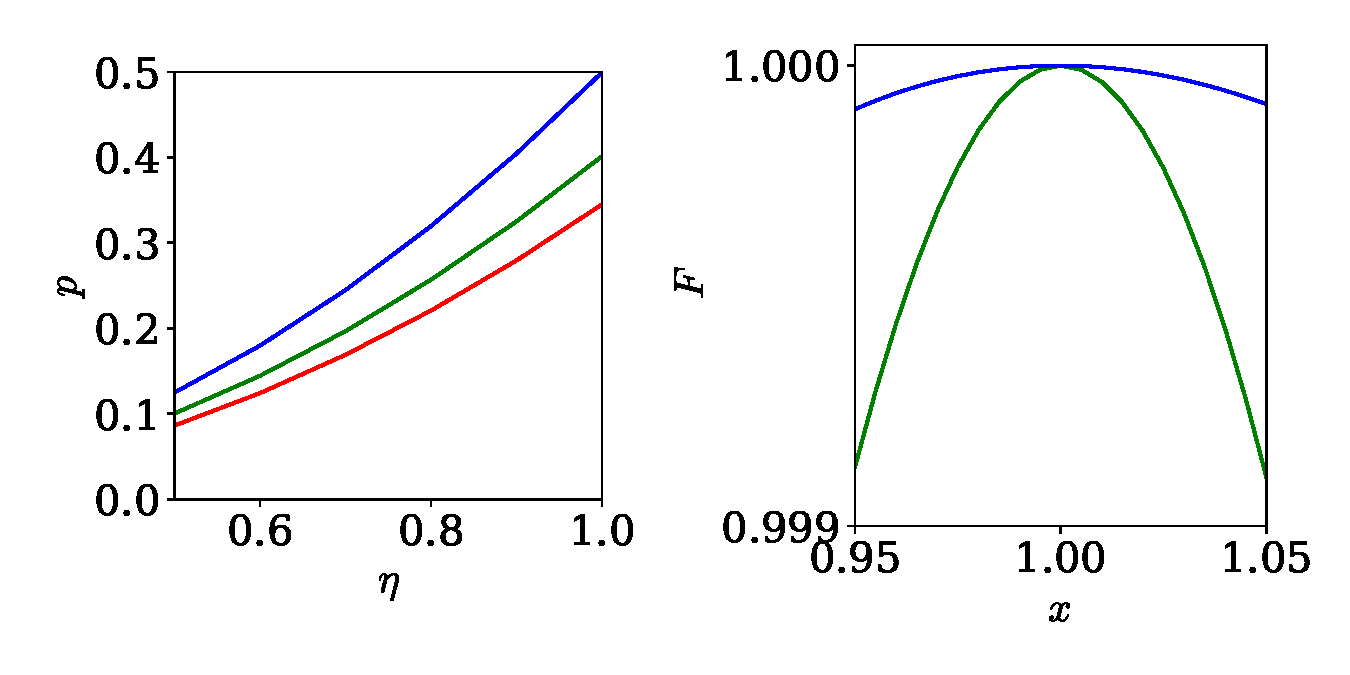
\includegraphics[width = 0.5 \linewidth]{figures/barett_fig2.pdf}
    \caption{Caption}
    \label{fig:my_label}
\end{figure}

\begin{figure}[H]
    \centering
    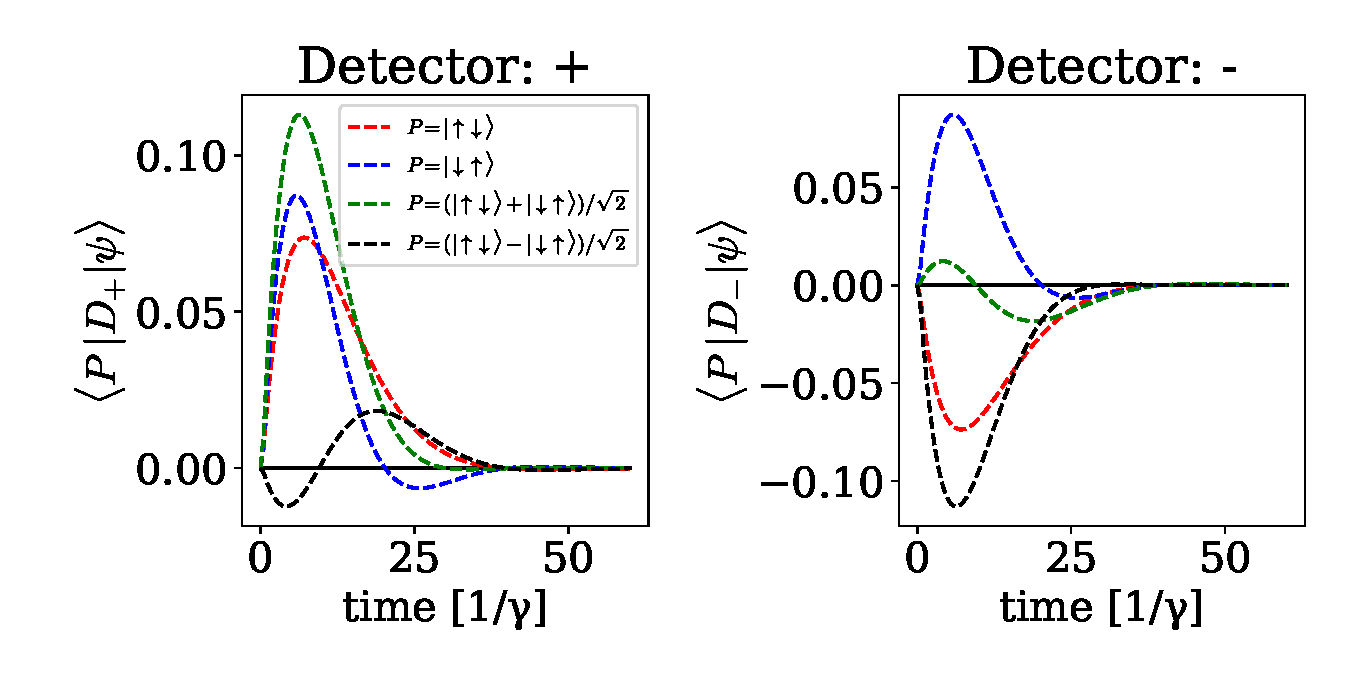
\includegraphics[width = 0.5 \linewidth]{figures/barett_uneven_g_first_detection.pdf}
    \caption{Uneven g, first round of detection.}
    \label{fig:my_label}
\end{figure}

\begin{figure}[H]
    \centering
    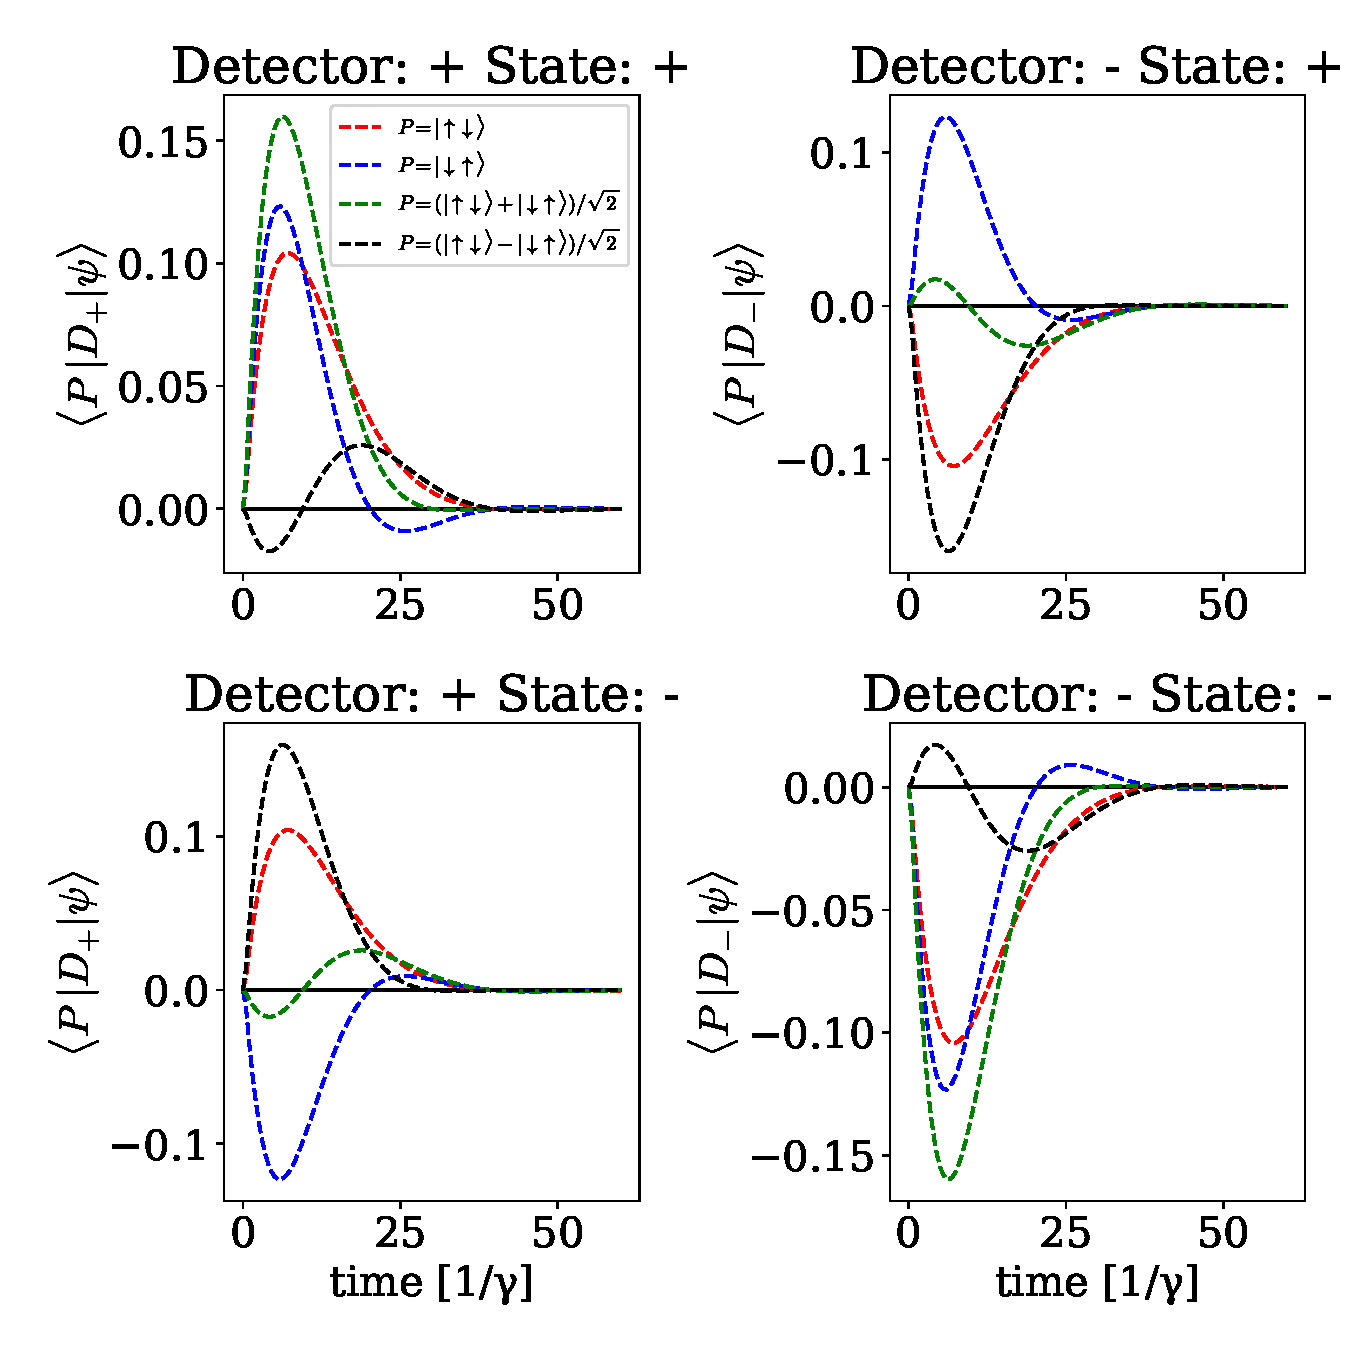
\includegraphics[width = 0.5 \linewidth]{figures/barett_uneven_g_second_detection.pdf}
    \caption{Uneven g, second round}
    \label{fig:my_label}
\end{figure}

\begin{figure}[H]
    \centering
    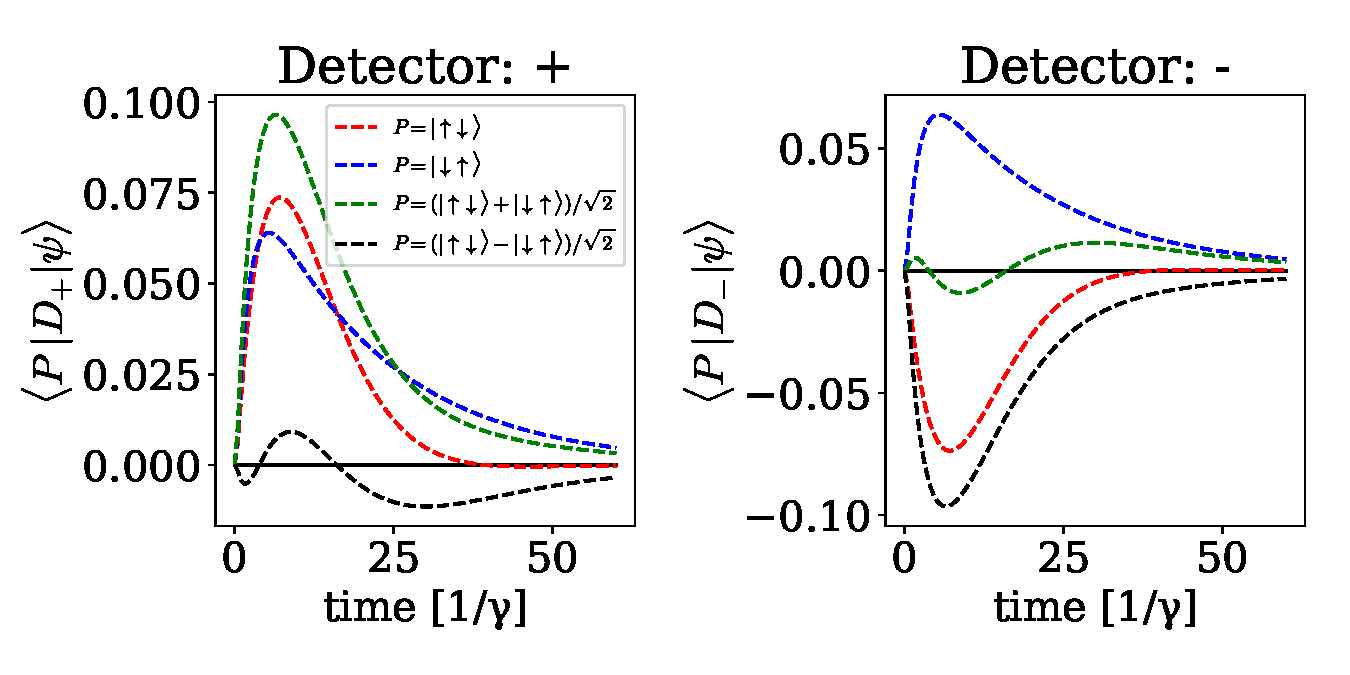
\includegraphics[width = 0.5 \linewidth]{figures/barett_uneven_kappa_first_detection.pdf}
    \caption{Uneven $\kappa$ first round}
    \label{fig:my_label}
\end{figure}

\begin{figure}[H]
    \centering
    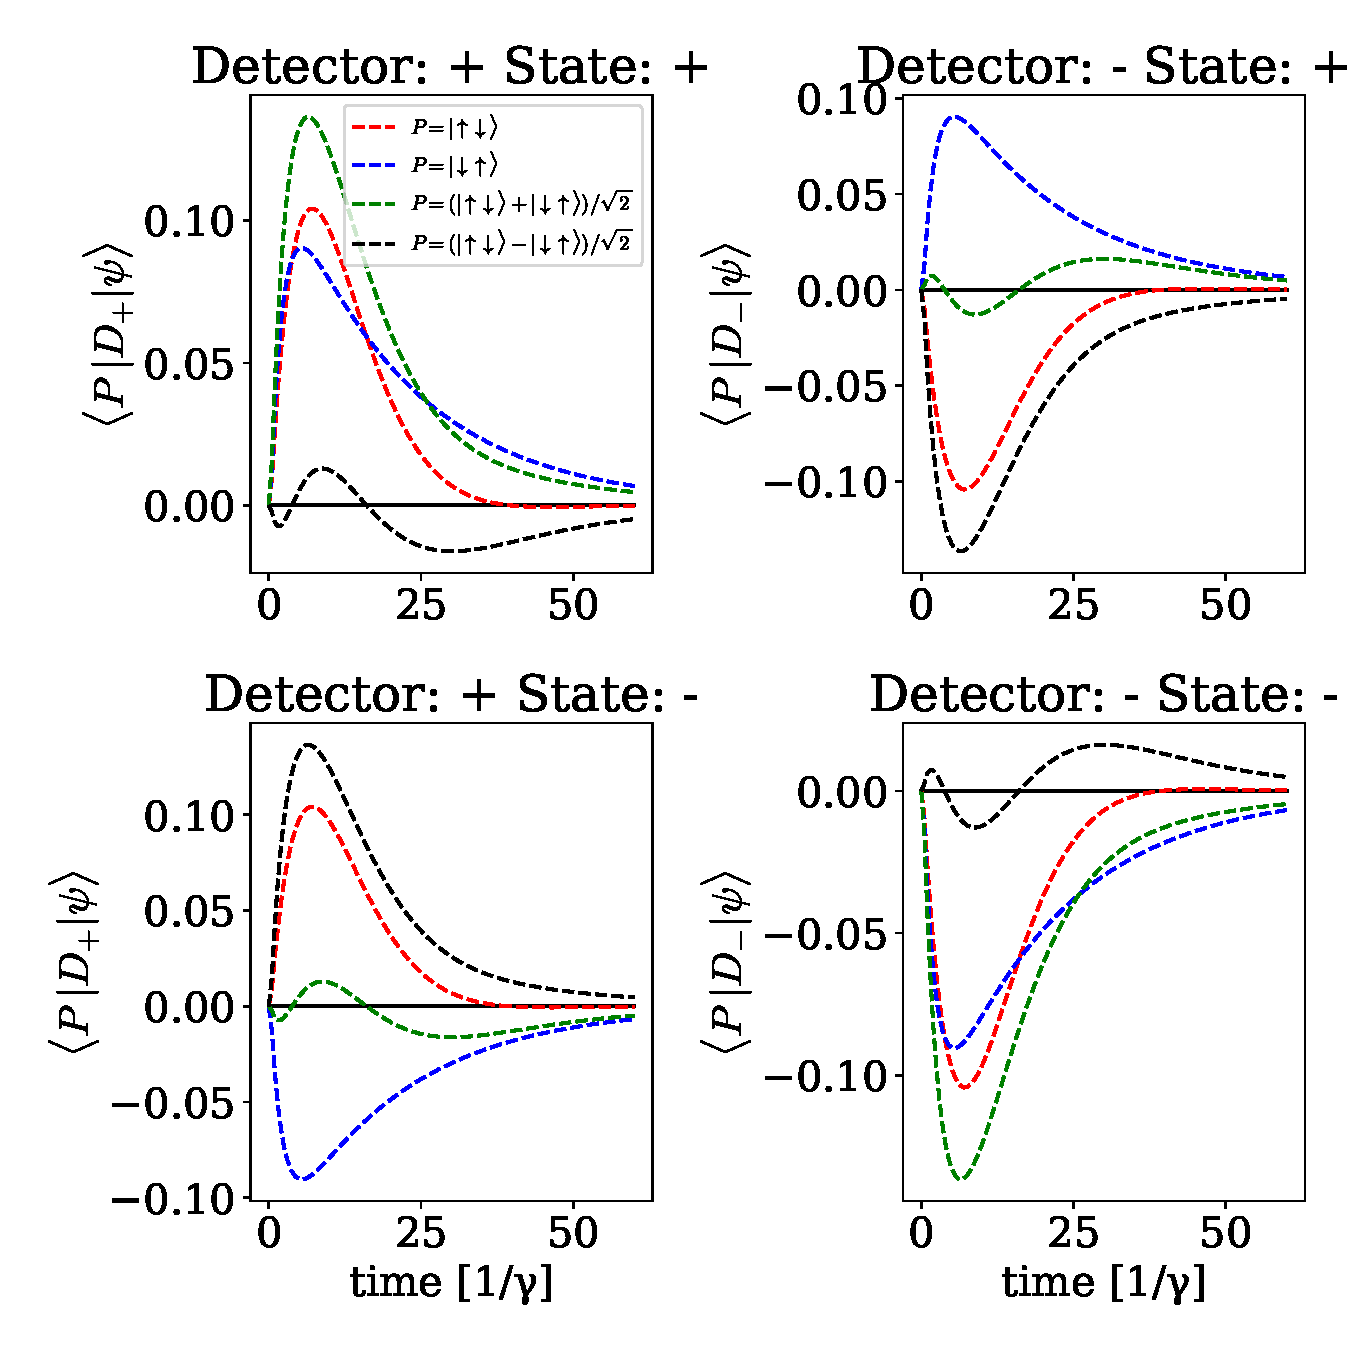
\includegraphics[width = 0.5 \linewidth]{figures/barett_uneven_k_second_detection.pdf}
    \caption{Uneven $\kappa$ second round}
    \label{fig:my_label}
\end{figure}


\section{Detection in waveguide using Monte-Carlo trajectories}

At each timeindex $t_k$ the interaction between the cavity and the waveguide is given by $i \sqrt{\gamma/dt} ( a w_k^\dagger - a^\dagger w_k)$ where $w_k$ is the annihilation operator for a photon in the waveguide in the timebin $t_k$. If we assume that the photon is detected in the waveguide the timebin after it was emitted (this seems reasonable?), the jump operator for the detection event is $w_{k-1}$. The jump operator would thus be changing at each timestep to be the annihilation operator for the previous step. Question is, what should the associated rate with this jump be? In this case we are not describing the leakage of a cavity but a photon hitting a detector. The intuitive answer to the rate would be the probablility of having a photon in that timebin times the timestep: $\abs{\xi_{k-1}}^2 \mathrm{dt}$ (with our state being $\ket{\psi}=\sum_k \sqrt{\mathrm{dt}}\ \xi_k w_k^\dagger \ket{\emptyset}$. But this is exactly just the overlap $\abs{\xi_{k-1}}^2=\expval{w_{k-1}^\dagger w_{k-1} }{\psi}/\mathrm{dt}$ which I guess is already included in the monte-carlo trajectory formalism? So maybe the rate is just unity (one). However, when I run simulations I notice that there is a high chance of no detection event happening at all! This should never be the case. We know that we will have a jump/detection, just not when the jump happens. This leads me to think that the above reasoning is wrong and that I'm missing something. Should the jump operator or rate somehow be cumulative so that we ensure that a jump happens or should the jump operator itself be different?

\section{Waveguide interactions}
If we consider two waveguides interacting we then have:
\begin{equation}
    H_{int} = V \left ( \int \frac{dk}{\sqrt{2 \pi}} \int \frac{dk'}{\sqrt{2 \pi}} w_{1}(k)^\dagger w_{2}(k') + \int \frac{dk}{\sqrt{2 \pi}} \int \frac{dk'}{\sqrt{2 \pi}} w_{2}(k')^\dagger w_{1}(k)\right )
\end{equation}
In the interaction picture with
\begin{equation}
    H_0 = \sum_\mu \int_{-\infty}^\infty d k k w^\dagger_\mu(k)w_\mu(k)
\end{equation}
we have the transformation: 
\begin{equation}
    \mathrm{e}^{i t H_0} w_\mu(k) \mathrm{e}^{-i t H_0} = \mathrm{e}^{-ikt} w_\mu(k)
\end{equation}
and thus:
\begin{equation}
    \mathrm{e}^{i H_0 t } H_{int} \mathrm{e}^{-i H_0 t } = V \left ( \int \frac{dk}{\sqrt{2 \pi}} \int \frac{dk'}{\sqrt{2 \pi}} \mathrm{e}^{ikt} w^\dagger_{1}(k) \mathrm{e}^{-ik't} w_{2}(k') + \int \frac{dk}{\sqrt{2 \pi}} \int \frac{dk'}{\sqrt{2 \pi}} \mathrm{e}^{ik't} w^\dagger_{2}(k') \mathrm{e}^{-ikt} w_{1}(k)\right )
\end{equation}
Introducing the fourier transformed operators $w_\mu(t) = \frac{1}{\sqrt{2 \pi}} \int_{-\infty}^\infty d k \mathrm{e}^{-ikt} w_{\mu}(k)$ we have: 
\begin{equation}
    H_{int}(t)  = \mathrm{e}^{i H_0 t } H_{int} \mathrm{e}^{-i H_0 t } = V \left ( w_1^\dagger(t) w_2(t) + w_2^\dagger(t) w_1(t)\right )
\end{equation}
Similarly, the unitary evolution operator becomes (for now let's exclude $H_s$ and $V(t)$):
\begin{equation}
    U_n = \mathrm{e}^{- i \int_{t_{n-1}}^{t_n} dt' H_{int}(t)} = \mathrm{e}^{- i \int_{t_{n-1}}^{t_n} dt' V \left ( w_1^\dagger(t') w_2(t') + w_2^\dagger(t') w_1(t')\right )}
\end{equation}
In previous examples we make the discretization:
\begin{equation}
    w_{\mu,n} = \frac{1}{\sqrt{\Delta t}} \int_{t_{n-1}}^{t_n} d t' w_{\mu}(t')
\end{equation}
And thus the natural extension would be:
\begin{equation}
    U_n = \mathrm{e}^{- i \Delta t V \left ( w^\dagger_{1,n} w_{2,n} + w_{2,n}^\dagger w_{1,n}\right )}
\end{equation}
But this is not equivalent since:
\begin{equation}
   \int_{t_{n-1}}^{t_n} dt' w_1^\dagger(t') w_2(t') \neq  w^\dagger_{1,n} w_{2,n} = \frac{1}{\sqrt{\Delta t}} \int_{t_{n-1}}^{t_n} d t' w^\dagger_{1}(t') \frac{1}{\sqrt{\Delta t}} \int_{t_{n-1}}^{t_n} d t' w_{2}(t')
\end{equation}





Defining then: 

\begin{align}
c_{\mathrm{in}}(t) & =\int \frac{d k}{\sqrt{2 \pi}} c_{\mathrm{in}, k}\left(t_0\right) e^{-i k\left(t-t_0\right)}, \\
c_{\mathrm{out}}(t) & =\int \frac{d k}{\sqrt{2 \pi}} c_{\mathrm{out}, k}\left(t_1\right) e^{-i k\left(t-t_1\right)},
\end{align}

with $t_0 \rightarrow - \infty$ and $t_1 \rightarrow \infty$

and thus equivalently:

\begin{align}
c_{\mathrm{in,k}}\left(t_0\right) & =\int \frac{d k}{\sqrt{2 \pi}} c_{\mathrm{in}}(t) e^{-i k\left(t-t_0\right)}, \\
c_{\mathrm{out,k}}\left(t_1\right) & =\int \frac{d k}{\sqrt{2 \pi}} c_{\mathrm{out}}(t) e^{-i k\left(t-t_1\right)},
\end{align}

$\int_{-1}^{1} e^{-(x-x_0)^2} dx = \frac{\sqrt{\pi}}{2} \left[ \mathrm{erf}\left(\frac{1-x_0}{\sqrt{2}}\right) - \mathrm{erf}\left(\frac{-1-x_0}{\sqrt{2}}\right) \right]
$


We get:

\begin{equation}
    H =  V \left ( \int \frac{dk}{\sqrt{2 \pi}} \int \frac{dk'}{\sqrt{2 \pi}} c_{in,k}^\dagger c_{out,k'} + \int \frac{dk}{\sqrt{2 \pi}} \int \frac{dk'}{\sqrt{2 \pi}} c_{out,k}^\dagger c_{in,k'} \right )
\end{equation}


\section{Waveguide Interaction}

Assume we have two waveguides with corresponding creation and annihilation operators $\omega_1$ and $\omega_2$. They interact via:
$$
\begin{aligned}
& H_I(t)=\sum_k f_k(t) V\left(w_1^{+}\left(t_k\right) w_2\left(t_k\right)+w_2^{+}\left(t_k\right) w_1\left(t_k\right)\right) \\
& \text { Where } f_k(t)= \begin{cases}1 \text { if } t=t_k \\
0 \text { else }\end{cases}
\end{aligned}
$$
We note that $\left[H_I(t), H_I\left(t^{\prime}\right)\right]=0$
That can probably be exploited in some way to show that we can do something like:
$$
\begin{aligned}
\quad \partial_t w_1\left(t_k\right) & = [ w_1,H_I ] = -\frac{i}{\hbar}\left[w_1\left(t_k\right), V\left(w_1^{\dagger}\left(t_k\right) w_2(t_k)+w_2^{\dagger}\left(t_k\right) w_1\left(t_k\right)\right)\right] \\
& =-\frac{i}{\hbar} V w_2\left(t_k\right)
\end{aligned}
$$
and $\quad \partial_t w_2\left(t_k\right)=-\frac{i}{\hbar} V w_1\left(t_k\right)$
Thus: $W=\left[\begin{array}{l}w_1\left(t_k\right) \\ w_2\left(t_k\right)\end{array}\right] \quad \partial_t W=\left(\begin{array}{cc}0 & -\frac{i}{\hbar} V \\ -\frac{i}{\hbar} V & 0\end{array}\right) W$

Furthermore we have:

$$
\begin{aligned}
&m:=\left[\begin{array}{cc}
0 & -\mathrm{I} V \\
-\mathrm{I} V & 0
\end{array}\right]\\
&\exp( M)=\left[\begin{array}{cc}
\cos (V) & -\mathrm{I} \sin (V) \\
-I \sin (V) & \cos (V)
\end{array}\right]
\end{aligned}
$$


\begin{equation}
    \ket{\psi} = \int_{t_0}^{t_{end}} \mathrm{d}t \ \xi_1(t) w_1^\dagger(t) \ket{\emptyset}_1\ket{\emptyset}_2 + \int_{t_0}^{t_{end}} \mathrm{d}t \ \xi_2(t) w_2^\dagger(t) \ket{\emptyset}_1\ket{\emptyset}_2
\end{equation}

\begin{equation}
    H = i \sqrt{\kappa_1/dt}(\sigma^\dagger w_1 - \sigma w_1^\dagger)+i \sqrt{\kappa_2/dt}(\sigma^\dagger w_2 - \sigma w_2^\dagger) + i V(w_1 ^\dagger w_2 - w_2^\dagger w_1) 
\end{equation}

\begin{equation}
    C_{lm}^{(2)}(t_1,t_2) = \abs{\psi_l(t_1)}^2 \abs{\psi_m(t_2)}^2
\end{equation}


\begin{align}
    & a \ket{n} = \sqrt{n} \ket{n-1} \\
    & a^\dagger \ket{n} = \sqrt{n+1} \ket{n+1}
\end{align}

\begin{align}
    \ket{n} = \begin{pmatrix} 0 \\ \vdots \\ 1  \\ \vdots \\ 0  \end{pmatrix}
\end{align}

\begin{align}
a = \begin{pmatrix}
0 & 0 & 0 & \cdots \\
1 & 0 & 0 & \cdots \\
0 & \sqrt{2} & 0 & \cdots \\
0 & 0 & \sqrt{3} & \cdots \\
\vdots & \vdots & \vdots & \ddots
\end{pmatrix}
\end{align}


$w_k^\dagger \ket{\emptyset} = \ket{1_k} \ \ \\ \ \\ $ 

$\frac{d}{dt} \mathbf{\Bar{x}} = \bar{\bar{a}} \mathbf{\Bar{x}}$ \ \ \\ \ \ \\ \ \

${H}\ket{\psi} = i\hbar\frac{\partial }{\partial t} \ket{\psi}$
